
\documentclass[11pt]{article}


%%%%%%%%%%%%%%%%%%%%%
%%%%%% Packages %%%%%
%%%%%%%%%%%%%%%%%%%%%

\usepackage[utf8]{inputenc}
\usepackage{booktabs}
\usepackage{amsmath}
\usepackage{amsfonts}
\usepackage{amssymb}
\usepackage{float}
\usepackage{color}
%\usepackage{appendix}
\usepackage{booktabs}
%\usepackage{etex}
\usepackage{microtype}
\usepackage{geometry}
\geometry{
	a4paper,
	left=20mm,
	top=20mm,
	right=20mm,
	bottom=20mm
}

%\usepackage[pdfborder={0 0 0},pdfusetitle]{hyperref}
%\usepackage{doi}
\usepackage{tikz}
\usepackage{pgfplots}
%\usepackage{imakeidx}
\usepackage{hyperref}
\usepackage{multirow}
\usepackage{setspace}
\usepackage{comment}
%\usepackage[labelformat=parens,labelsep=quad,skip=3pt]{caption}
\usepackage{graphicx}
\usepackage{caption}
\usepackage{subcaption}
\usepackage{stata}

\usepackage{tabularx}

\usepackage{enumitem}

\usepackage{adjustbox}

%%%%%%%%%%%%%%%%%%%%%
%%%%%% Document %%%%%
%%%%%%%%%%%%%%%%%%%%% 


\title{Pakistan Police Project: \\ Data Exploration Notes}
\date{\today}

\begin{document}
	
\maketitle

This document provides notes on our exploration of the Complaints and First Impression Reports data.

\section{Dataset Overview}

The numbers of unique observations for each of the FIR and Complaint datasets are the following: \\
\noindent Unique Complaints cases $\rightarrow$  154058 \\
\noindent Unique FIR cases $\rightarrow$ 2255694

The merged FIR + Complaint dataset looks like this. The ``In both" category shows the unique matched observations between the two datasets.
\begin{table}[!h]
\caption{Match between the FIR and Complaint Data}
\centering
\begin{tabular}{lll}
\cline{1-3}
\multicolumn{1}{c}{} &
  \multicolumn{1}{|r}{Frequency} &
  \multicolumn{1}{r}{Percent} \\
\cline{1-3}
\multicolumn{1}{l}{Data source} &
  \multicolumn{1}{|r}{} &
  \multicolumn{1}{r}{} \\
\multicolumn{1}{l}{\hspace{1em}FIR} &
  \multicolumn{1}{|r}{2,112,426} &
  \multicolumn{1}{r}{93.20} \\
\multicolumn{1}{l}{\hspace{1em}Complaints (Lahore)} &
  \multicolumn{1}{|r}{10,790} &
  \multicolumn{1}{r}{0.48} \\
\multicolumn{1}{l}{\hspace{1em}In both} &
  \multicolumn{1}{|r}{143,268} &
  \multicolumn{1}{r}{6.32} \\
\multicolumn{1}{l}{\hspace{1em}Total} &
  \multicolumn{1}{|r}{2,266,484} &
  \multicolumn{1}{r}{100.00} \\
\cline{1-3}
\end{tabular}
\end{table}



\section{Response Speed}

These are summary statistics on police response seped. 

Once thing to note is that there are quit a bit of negative values. 

	\begin{table}[htbp]\centering
\def\sym#1{\ifmmode^{#1}\else\(^{#1}\)\fi}
\caption{Response Speed}
\begin{tabular}{l*{1}{ccccc}}
\hline\hline
                    &\multicolumn{5}{c}{}                                            \\
                    &       count&         min&         max&         p50&        mean\\
\hline
Complaint-1st Contact Time (hours)&      143268&   -.0197222&    2726.877&    10.16653&     39.7748\\
Complaint-FIR convertion time (hours)&      143268&   -26347.93&    16247.58&   -.3427778&    1.866467\\
\hline
Observations        &      143268&            &            &            &            \\
\hline\hline
\end{tabular}
\end{table}

	
Without negative values, the summary statistics look like this.

	\begin{table}[htbp]\centering
\def\sym#1{\ifmmode^{#1}\else\(^{#1}\)\fi}
\caption{Response Speed}
\begin{tabular}{l*{1}{ccccc}}
\hline\hline
                    &\multicolumn{5}{c}{}                                            \\
                    &       count&         min&         max&         p50&        mean\\
\hline
Complaint-1st Contact Time (hours)&       68871&       .0075&    2726.877&    50.05167&    71.81699\\
Complaint-FIR convertion time (hours)&       68871&    6.78e-11&    16247.58&    34.64444&    60.28819\\
\hline
Observations        &       68871&            &            &            &            \\
\hline\hline
\end{tabular}
\end{table}

	

Here are the distributions. I cut off some outliers so that we can see some patterns. 

A question: Why do we see some waves? 

	\begin{figure}[H]
		\centering
		\caption{Estimated Effects: All Treatment Categories}
		\begin{subfigure}[b]{0.49\textwidth}
			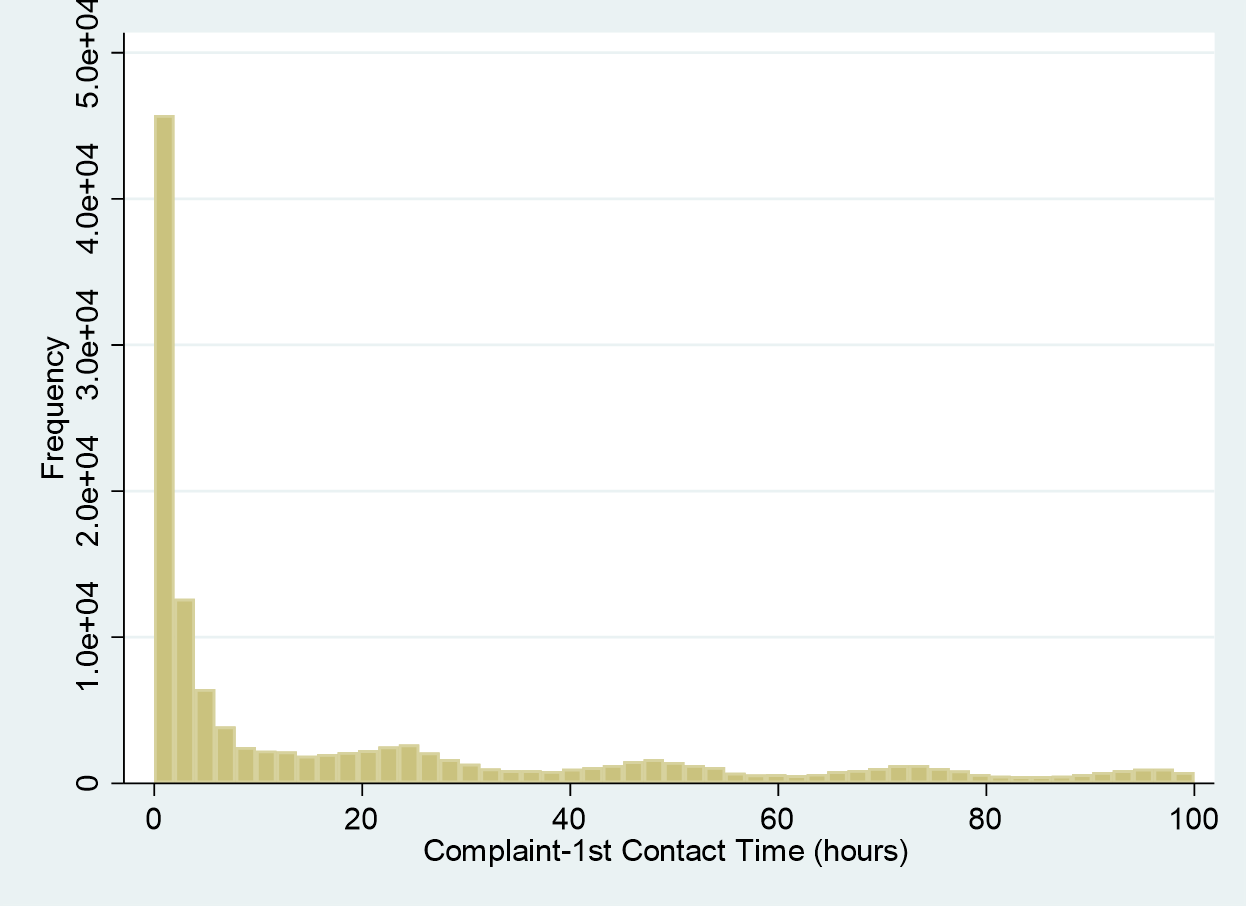
\includegraphics[width=\textwidth]{Hist_responsetime}
			\label{fig:Hist_responsetime}
		\end{subfigure}
		%
		\begin{subfigure}[b]{0.49\textwidth}
			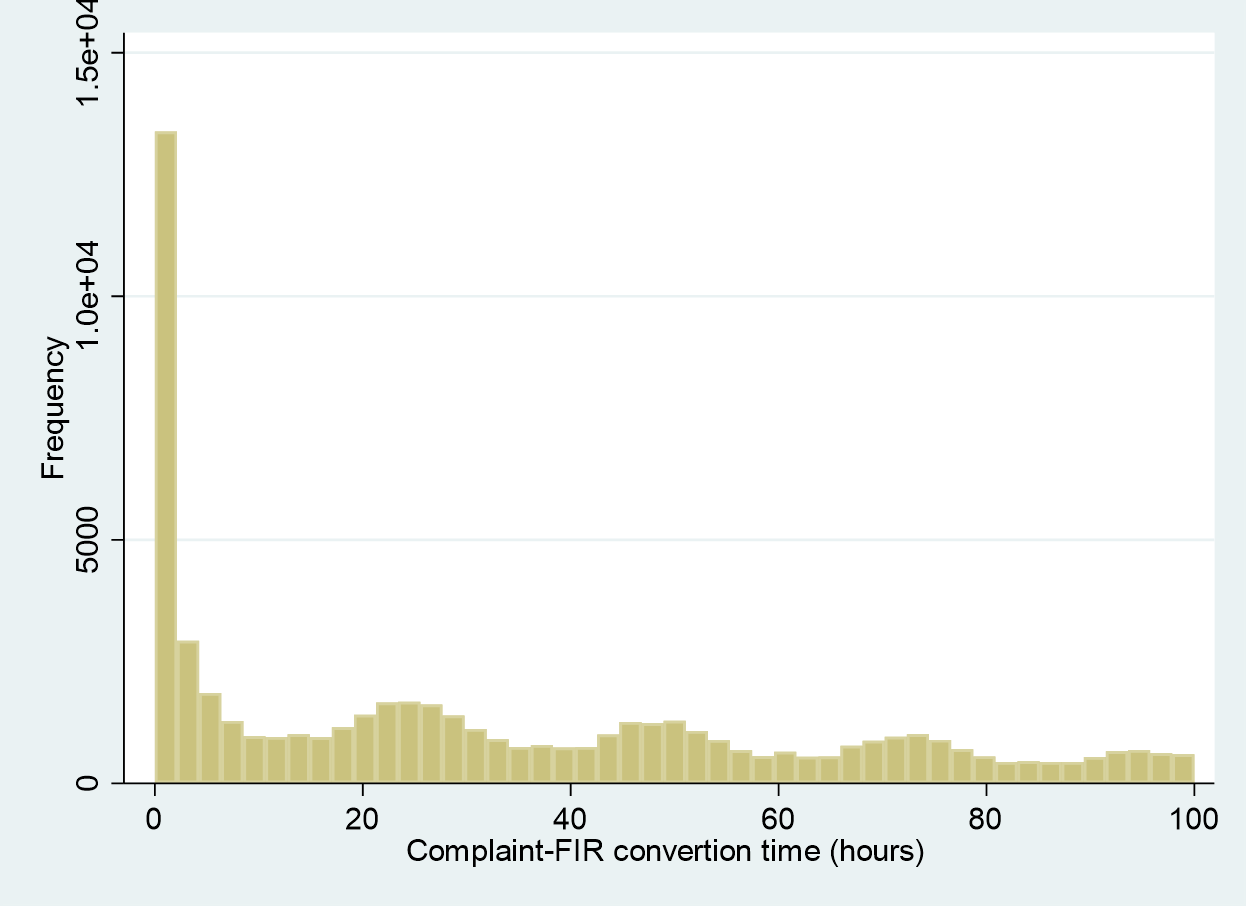
\includegraphics[width=\textwidth]{Hist_timeComp2Fir}
			\label{fig:Hist_timeComp2Fir}
		\end{subfigure}
	\end{figure}
	
%\begin{table}[H]
%\adjustbox{max width=\textwidth}{
%\input{Effects_Updating_Other_exp_donate_pmcf}
%}
%\end{table}

						    
%\begin{figure}[H]
%\centering
%\caption{Estimated Effects: All Treatment Categories}
%\begin{subfigure}[b]{0.49\textwidth}
%	\includegraphics[width=\textwidth]{Effects_AllTreatCats_exp_donate_pmcf}
%	\label{fig:checkattenbeforeaug22}
%\end{subfigure}
%
%\begin{subfigure}[b]{0.49\textwidth}
%	\includegraphics[width=\textwidth]{Effects_AllTreatCats_exp_vote_bjp_if}
%	\label{fig:checkattenafteraug22}
%\end{subfigure}
%\medskip
%\begin{subfigure}[b]{0.49\textwidth}
%	\includegraphics[width=\textwidth]{Effects_AllTreatCats_exp_vote_bjp_lkl_more}
%	\label{fig:checkattenbeforeaug22}
%\end{subfigure}
%
%\begin{subfigure}[b]{0.49\textwidth}
%	\includegraphics[width=\textwidth]{Effects_AllTreatCats_exp_vote_nda_if}
%	\label{fig:checkattenafteraug22}
%\end{subfigure}
%
%\end{figure}

\end{document}

